\documentclass[border=6pt]{standalone}
\usepackage{fontspec,unicode-math}
\setmainfont{Noto Serif}
\setmathfont{STIXTwoMath-Regular.otf}
\usepackage{tikz}
\usetikzlibrary{arrows.meta,calc,patterns,decorations.markings,decorations.pathmorphing,decorations.pathreplacing}
\tikzset{lev/.style={line width=1.2pt,line cap=butt},
 fine/.style={line width=.54pt},light/.style={line width=.37pt},
 curve/.style={line width=1.2pt,line cap=round,line join=round},
 ax/.style={line width=.62pt,-{Latex[length=2.1mm,width=1.15mm]}},
 ray/.style={line width=.58pt,-{Latex[length=1.85mm,width=.95mm]},shorten >=1.4pt,shorten <=1.4pt},
 dim/.style={line width=.52pt,{Latex[length=1.6mm,width=.85mm]}-{Latex[length=1.6mm,width=.85mm]}},
 flow/.style={line width=.60pt,postaction={decorate},decoration={markings,mark=at position .62 with {\arrow{Latex[length=1.8mm,width=.95mm]}}}},
 lab/.style={font=\fontsize{12}{14.4}\selectfont,inner sep=1.6pt},
 small/.style={font=\fontsize{10.5}{12.5}\selectfont,inner sep=1.3pt},
 tinylabel/.style={font=\fontsize{9.2}{11}\selectfont,inner sep=1.0pt},
 panel/.style={font=\fontsize{12}{14.4}\selectfont\itshape,inner sep=1.5pt}}
\pagestyle{empty}
\begin{document}
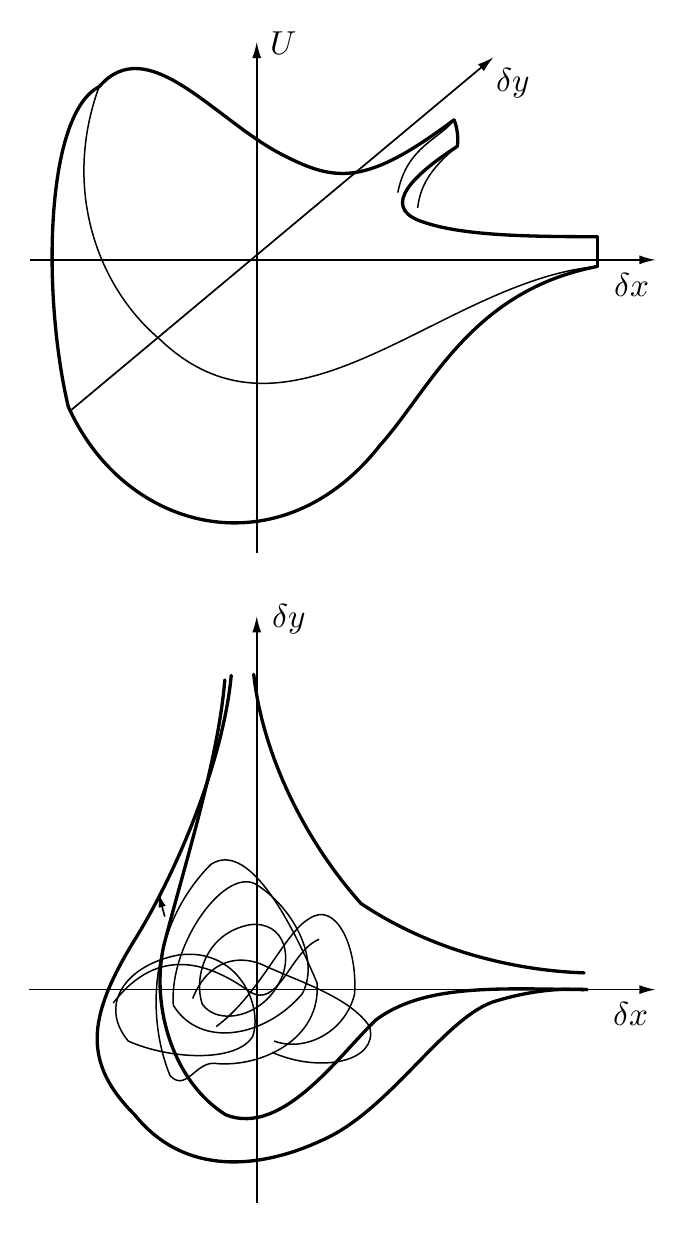
\begin{tikzpicture}[x=1cm,y=1cm,line join=round]
\draw[ax] (0.54800,12.54400)--(8.50000,12.54400);
\node[lab,anchor=north east] at (8.48600,12.44600) {$\delta x$};
\draw[ax] (3.43200,8.82000)--(3.43200,15.31600);
\node[lab,anchor=west] at (3.54400,15.28800) {$U$};
\draw[ax] (1.08000,10.64000)--(6.44200,15.12000);
\node[lab,anchor=north west] at (6.41400,15.05000) {$\delta y$};
\draw[curve] (1.03800,10.68200) .. controls (0.70200,12.11000) and (0.74400,14.39200) .. (1.43000,14.74200);
\draw[curve] (1.43000,14.74200) .. controls (2.04600,15.45600) and (2.88600,14.33600) .. (3.74000,13.88800);
\draw[curve] (3.74000,13.88800) .. controls (4.44000,13.52400) and (4.81800,13.48200) .. (5.93800,14.32200);
\draw[curve] (5.93800,14.32200) .. controls (5.98000,14.22400) and (5.99400,14.08400) .. (5.98000,13.98600);
\draw[curve] (5.98000,13.98600) .. controls (5.26600,13.52400) and (5.05600,13.17400) .. (5.56000,13.02000);
\draw[curve] (5.56000,13.02000) .. controls (6.05000,12.85200) and (6.87600,12.83800) .. (7.75800,12.83800);
\draw[curve] (7.75800,12.83800)--(7.75800,12.46000);
\draw[curve] (7.75800,12.46000) .. controls (6.14800,12.15200) and (5.63000,10.89200) .. (5.00000,10.19200);
\draw[curve] (5.00000,10.19200) .. controls (3.75400,8.59600) and (1.76600,9.05800) .. (1.03800,10.68200);
\draw[fine] (1.43000,14.74200) .. controls (0.95400,13.44000) and (1.41600,12.19400) .. (2.20000,11.53600);
\draw[fine] (2.20000,11.53600) .. controls (3.88000,9.92600) and (5.77000,12.27800) .. (7.75800,12.46000);
\draw[fine] (5.98000,13.98600) .. controls (5.61600,13.69200) and (5.50400,13.45400) .. (5.47600,13.20200);
\draw[fine] (5.93800,14.32200) .. controls (5.77000,14.08400) and (5.33600,13.98600) .. (5.22400,13.39800);
\node[panel] at (1.19200,8.75000) {а};
\draw[ax] (0.53400,3.27600)--(8.50000,3.27600);
\node[lab,anchor=north east] at (8.47200,3.17800) {$\delta x$};
\draw[ax] (3.43200,0.56000)--(3.43200,8.02200);
\node[lab,anchor=west] at (3.57200,7.98000) {$\delta y$};
% CP11: source-guided lower-panel multiple intersecting loops.
% A qualitative projection of a trajectory; no claim of integrating the flow.
\draw[curve] (3.1082,7.2662) .. controls (3.0128,6.2296) and (2.4544,4.8238) .. (1.8688,3.8866) .. controls (1.2695,2.9068) and (1.2286,2.3388) .. (1.8824,1.6856) .. controls (2.5361,0.8762) and (3.5168,1.0182) .. (4.2523,1.3590) .. controls (5.1103,1.7282) and (5.7913,2.8926) .. (6.4315,3.1198) .. controls (6.9763,3.2902) and (7.3712,3.2902) .. (7.6300,3.2760);
\draw[curve] (3.3942,7.2804) .. controls (3.5032,6.2722) and (4.0343,5.1788) .. (4.7562,4.3694) .. controls (5.6687,3.7588) and (6.7311,3.5174) .. (7.5892,3.4890);
\draw[curve] (3.0265,7.2094) .. controls (2.9447,6.2012) and (2.5361,4.9374) .. (2.2501,3.8298) .. controls (2.0867,3.0772) and (2.3591,2.1116) .. (3.0401,1.6856) .. controls (3.7619,1.4016) and (4.4838,2.4524) .. (4.9469,2.8926) .. controls (5.5598,3.3470) and (6.4859,3.2902) .. (7.5892,3.2760);
\draw[fine] (2.3318,2.1826) .. controls (1.9913,3.0204) and (2.1275,4.1422) .. (2.8494,4.8664) .. controls (3.3670,5.2072) and (3.9526,3.9434) .. (4.1978,3.3612) .. controls (4.2523,2.6370) and (3.4759,2.2820) .. (2.9039,2.3388) .. controls (2.6587,2.3672) and (2.5361,1.9696) .. (2.3318,2.1826);
\draw[fine] (1.8007,2.6228) .. controls (1.4193,3.0772) and (1.7598,3.5884) .. (2.4408,3.7162) .. controls (3.1899,3.8156) and (3.5168,3.0772) .. (3.3806,2.6796) .. controls (3.1627,2.3388) and (2.3046,2.3956) .. (1.8007,2.6228);
\draw[fine] (2.3727,3.0772) .. controls (2.3182,3.8866) and (3.0673,4.8806) .. (3.4487,4.5966) .. controls (3.9254,4.2842) and (4.2386,3.6310) .. (4.0071,3.2192) .. controls (3.5304,2.6654) and (2.7132,2.5234) .. (2.3727,3.0772);
\draw[fine] (2.7404,3.0914) .. controls (2.6315,3.4180) and (2.7677,3.9860) .. (3.3397,4.0996) .. controls (3.8028,4.1564) and (3.8981,3.6594) .. (3.7075,3.3470) .. controls (3.4895,2.9352) and (2.9447,2.8074) .. (2.7404,3.0914);
\draw[fine] (2.6179,3.1624) .. controls (2.8222,3.6736) and (3.2308,3.7304) .. (3.5440,3.5742) .. controls (3.9799,3.3754) and (4.6200,3.1766) .. (4.8652,2.8074) .. controls (4.9877,2.3530) and (4.2250,2.2110) .. (3.6257,2.4808);
\draw[fine] (2.9175,2.8074) .. controls (3.4623,3.2050) and (3.7892,4.0002) .. (4.0888,4.1706) .. controls (4.4429,4.4262) and (4.7153,3.8014) .. (4.6745,3.2192) .. controls (4.5519,2.7222) and (4.0343,2.4808) .. (3.6530,2.6228);
\draw[fine] (1.6100,3.1056) .. controls (2.1956,3.8724) and (2.8630,3.5884) .. (3.3261,3.2618) .. controls (3.7075,2.9920) and (3.8573,3.7730) .. (4.2250,3.9150);
\draw[ray] (2.2774,4.1564)--(2.1684,4.5540);
\node[panel] at (1.19200,0.65800) {б};
\end{tikzpicture}
\end{document}
